\section{Ralph Munday Denton-Barker}\label{Ralph_Munday_Denton-Barker}

\begin{center}
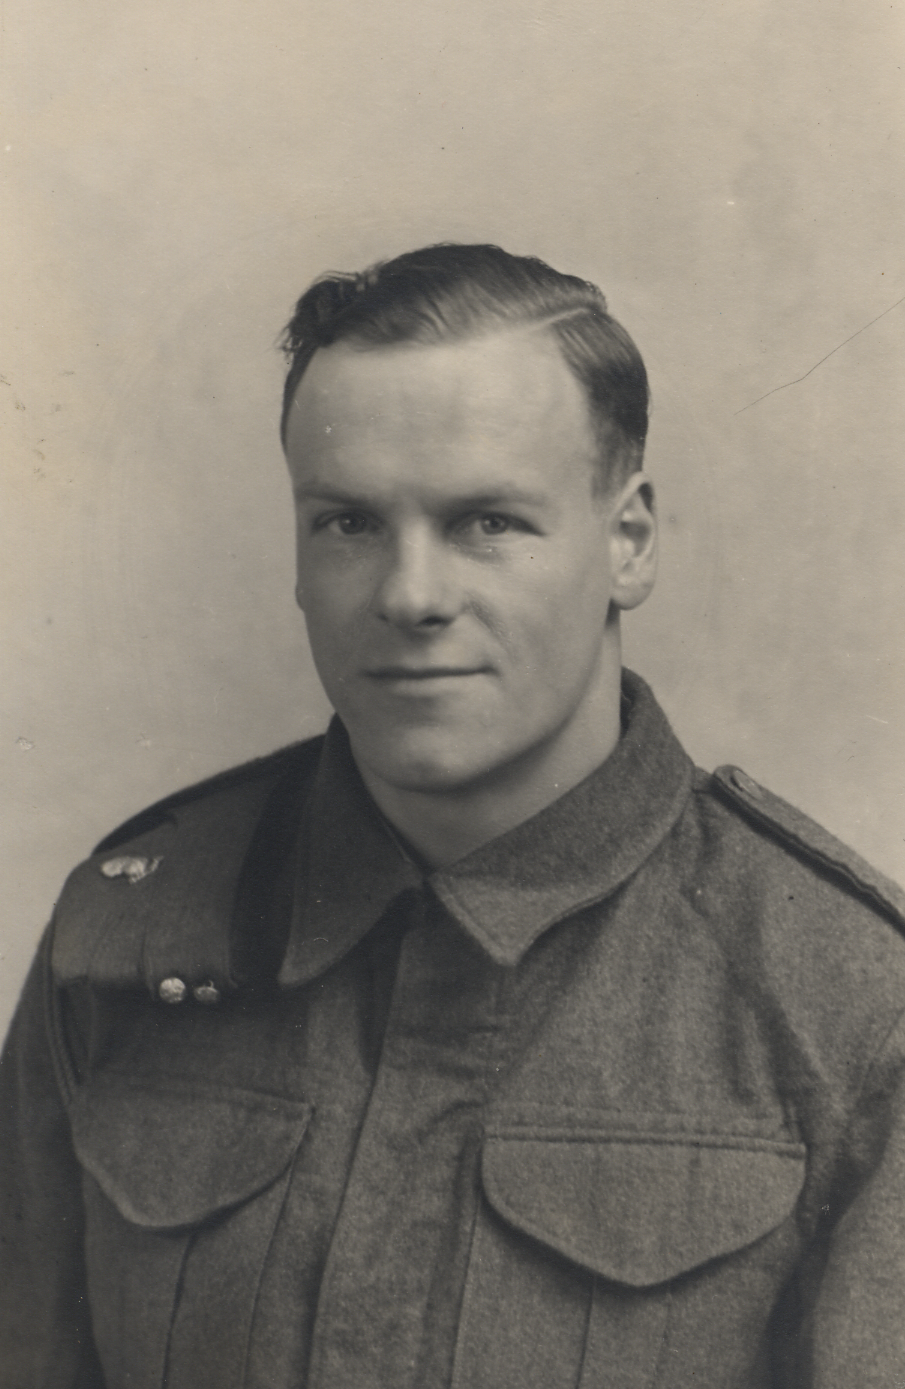
\includegraphics[width=0.8\linewidth]{photos/Ralph_Munday_Denton-Barker} \\
{\footnotesize c. 1935\cite{FlickrTeachers}}
\end{center}

\textbf{Ralph Denton-Barker} (17 July 1916 -- 4 November 1990) was born in 1916 in Birkenhead \cite{BMDIndex_RalphMundayDentonBarker_birth} where he grew up with his older brother Mead and yonger sister Virginia (p.\pageref{Virginia_Kathleen_Denton_Barker}).

Ralph was educated at Cheam and Felsted, and Birkenhead School. He joined the Alliance Insurance Company to train as an actuary, but left the company on joining the army at the beginning of the war. He served as a Private soldier throughout the war, and after demobilisation he trained as a primary school teacher, and worked as a teacher in Bedfordshire (living at the Old Schoolhouse in Pertenhall), Worcestershire (living at Dove Cottage, Great Witley and teaching at Arley Kings Primary School) and then in Cornwall (living at The Barn, Portloe and teaching at Mevagissey until he retired in 1970). He and his wife Nyria (they married on 28 June 1947 in Edmonton, Middlesex \cite{MarriageCertRalphDentonBarkerJoanNyriaPowell} bought a farm in West Penwith in 1965 and they farmed (dairy and beef, at Kerrow Farm) until they moved to Menorca where they had a small holding (known as a finca) outside Alayor. They then moved to C'an Amoros, outside Pollensa in Mallorca where Ralph had a few cows and a large citrus orchard.

They moved to Australia in 1978, on a Russian ship (via Sri Lanka, arriving on March 17th), and after a year in Western Australia (on Lapko's Farm, Denmark) they settled in Tasmania at Riverside Cottage, Upper Scamander, on the east coast.

He died on 4 November 1990, at home.
